\documentclass[tikz,border=5pt]{standalone}
\usepackage{xcolor}
\usepackage{amsmath}
\usepackage{amssymb}
\usetikzlibrary{positioning, arrows.meta, calc, fit, backgrounds,
  decorations.pathreplacing, shapes.geometric, shapes.symbols}
\begin{document}
\color{white}
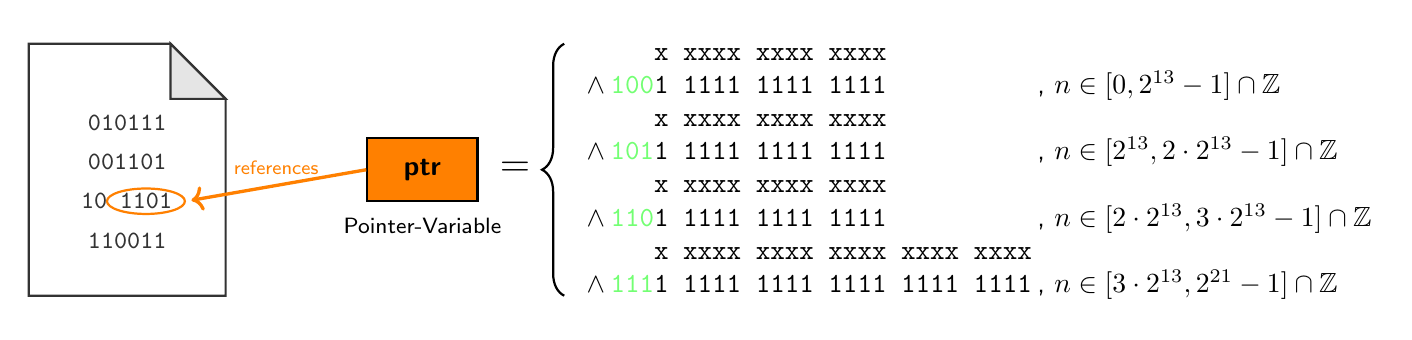
\begin{tikzpicture}
	\tikzset{
		binary file icon/.pic={
			\draw[fill=white, draw=black!80, thick]
			(0,0) -- (0,3.2) -- (1.8,3.2) -- (2.5,2.5) -- (2.5,0) -- cycle;
			\draw[fill=gray!20, draw=black!80, thick]
			(1.8,3.2) -- (1.8,2.5) -- (2.5,2.5) -- cycle;
			\node[minimum width=2.5cm, minimum height=3.2cm, inner sep=0, outer sep=0] (-box) at (1.25, 1.6) {};
			\node[font=\ttfamily\small, text=black!80] at (1.25, 2.2) {010111};
			\node[font=\ttfamily\small, text=black!80] at (1.25, 1.7) {001101};
			\node[font=\ttfamily\small, text=black!80, anchor=east] (p1) at (1.12, 1.2) {10};
			\node[draw=orange, thick, ellipse, inner sep=0.5pt, font=\ttfamily\small, text=black!80, right=-4pt of p1, anchor=west] (-meinkreis) {1101};
			\node[font=\ttfamily\small, text=black!80] at (1.25, 0.7) {110011};
		}
	}
	\pic (mem) at (0,-5) {binary file icon};
	\node[draw, rectangle, minimum width=1.4cm, minimum height=0.8cm, fill=orange, text=black, thick, font=\sffamily\bfseries] (ptr) at (5, -3.4) {ptr};
	\node[font=\sffamily\footnotesize, below=2pt of ptr] {Pointer-Variable};
	\draw[->, very thick, orange, shorten >=2pt]
	(ptr.west) -- node[above, font=\sffamily\scriptsize] {references} (mem-meinkreis.east);
	\draw[thick, decorate, decoration={brace, mirror, amplitude=8pt}]
	([xshift=4.3cm]mem-box.north east) -- ([xshift=4.3cm]mem-box.south east)
	node[midway, left=0.3cm, font=\sffamily] {\textbf{\Large$=$}}
	node[midway, right=0cm,font=\sffamily] {
		\fontsize{10pt}{12pt}\selectfont
		\setlength{\tabcolsep}{1pt}
		\begin{tabular}{l l l}
			&\texttt{\ \ \ x xxxx xxxx xxxx}&\\
			$\land$&\texttt{\textcolor{green!55!white}{100}1 1111 1111 1111}&, $n\in [0,2^{13}-1]\cap \mathbb{Z}$\\
			&\texttt{\ \ \ x xxxx xxxx xxxx}&\\
			$\land$&\texttt{\textcolor{green!55!white}{101}1 1111 1111 1111}&, $n\in [2^{13},2 \cdot 2^{13}-1]\cap \mathbb{Z}$\\
			&\texttt{\ \ \ x xxxx xxxx xxxx}&\\
			$\land$&\texttt{\textcolor{green!55!white}{110}1 1111 1111 1111}&, $n\in [2 \cdot 2^{13},3 \cdot 2^{13}-1]\cap \mathbb{Z}$\\
			&\texttt{\ \ \ x xxxx xxxx xxxx xxxx xxxx}&\\
			$\land$&\texttt{\textcolor{green!55!white}{111}1 1111 1111 1111 1111 1111}&, $n\in [3 \cdot 2^{13},2^{21}-1]\cap \mathbb{Z}$
		\end{tabular}
	};
\end{tikzpicture}
\end{document}